% Version 2017-10-26
% update 170821 Affiliation list with numbers (Copernicus)
% update – 161114 by Ken Arroyo Ohori: made spacing closer to Word template throughout, put proper quotes everywhere, removed spacing that could cause labels to be wrong, added non-breaking and inter-sentence spacing where applicable, removed explicit newlines

\documentclass{isprs}
\usepackage{subfigure}
\usepackage{setspace}
\usepackage{geometry} % added 27-02-2014 Markus Englich
\usepackage{epstopdf}
\usepackage{multirow}
\usepackage[labelsep=period]{caption}  % added 14-04-2016 Markus Englich - Recommendation by Sebastian Brocks

\geometry{a4paper, top=25mm, left=20mm, right=20mm, bottom=25mm, headsep=10mm, footskip=12mm} % added 27-02-2014 Markus Englich
%\usepackage{enumitem}

%\usepackage{isprs}
%\usepackage[perpage,para,symbol*]{footmisc}

%\renewcommand*{\thefootnote}{\fnsymbol{footnote}}
\captionsetup{justification=centering} % thanks to Niclas Borlin 05-05-2016


\begin{document}

\title{COMPARING REGRESSION MODELS FOR PREDICTING PLANT NITROGEN CONTENT WITH HYPERSPECTRAL UAV DATA}


\author{Thomas Oosterhuis - 952805625020}


\address{Advanced Earth Observation 2018}

\workinggroup{} %This field is optional.
\icwg{}   %This field is optional.

\abstract{ 
The influence of nitrogen content on a plant's reflectance is poorly understood. A common regression method to predict plant traits from full hyperspectral reflectance is partial least squares regression (PLS). I compare the performance of ridge regression (RR) and random forest regression (RF) on predicting oat nitrogen content from hyperspectral UAV data with PLS. Both models outperform PLS. RR performs best on the validation set (RMSE = 2.01). RF is the most robust model during 8-fold CV (SD SSE = 2.81), due to its ensemble learning. There is high variable importance in the visible blue region. The different treatments of oat plots are apparent beyond 700nm. RR and RF are promising models for predicting plant traits from hyperspectral data. Future research should focus on feature selection and better insight in important spectral regions.
}

\keywords{Remote Sensing, Hyperspectral Data, Machine Learning, Regression, Multivariate Analysis, Biophysical Plant Traits}

\maketitle

\section{INTRODUCTION}
%\sloppy

In the 1960s, remote sensing emerged as a tool for characterising vegetation \cite{Houborg2015}. It led to the discovery that a plants' physical traits affect the reflectance of solar radiation on certain wavelengths of the spectral signature \cite{Knipling1970}. Using spectral information, it is possible to estimate parameters of plants' leaf biochemistry such as water, chlorophyll and nitrogen contents \cite{Hansen2003,Thorp2015}. Accurate estimation of such features is of fundamental importance for plant phenotyping, yield prediction and assessing plant conditions \cite{Diaz2016,Jay2017}. One difficulty in spectral analysis is that relations between reflectance and some plant traits are better understood than others. Nitrogen's relation to reflectance is partially unknown, even though plant nitrogen content is linked to chlorophyll content through photosynthesis. Leaf chlorophyll content influences reflectance in the green and red regions of the visible electromagnetic spectrum. Many vegetation indices (VIs) are developed to estimate chlorophyll presence using specific wavelengths. Examples are the red-edge index and the normalised difference vegetation index (NDVI), which use the visible red and near-infrared (NIR) region of the spectrum \cite{Elarab2015,Kooistra2016,Xue2017}. For cereals, VIs outperform on chlorophyll prediction compared to nitrogen prediction, which may indicate that the relation between nitrogen and reflection cannot be captured by a linear ratio \cite{Li2010}. Nitrogen is a limiting nutrient for crops. Accurate prediction of nitrogen content is useful for optimising fertiliser application in precision agriculture. With imaging spectroscopy reflectance in many contiguous wavelengths are measured ($<$ 5nm). By optimising wavelength selection, imaging spectroscopy can enhance the predictive performance of VIs, which improves understanding of plant traits and reflectance. Yet, by not investigating the entire hyperspectral reflectance, relevant information about plant traits may be missed \cite{Hansen2003}. Examining the predictive power of the entire hyperspectral reflectance on nitrogen content can thus lead to novel insights \cite{Hansen2003,Kitchen2010,Mulla2013,Nasi2017}.

\vspace{4mm}

A common statistical method to identify and quantify the relation between variables is regression, used to create a predictive model. A regression predicts a dependent variable (plant trait) through a number of independent variables (reflectances at certain wavelengths). The standard approach in a regression analysis is linear ordinary least squares (OLS), which minimises the sum of the squares of the residuals to estimate the coefficients of the independent variables. OLS requires more data points ($n$) than variables ($p$). However, with the narrow bandwidth measurements of hyperspectral imagery $p >> n$.  Because of the collinearity in predictors, there is no unique solution for OLS. Multiple solutions could yield a training error of zero and result in a highly variant model. The noise caused by collinearity also affects interpretation of the coefficient estimates for variable importance \cite{Stewart1987}. One method circumventing collinearity is partial least squares (PLS) regression, which is widely used for hyperspectral analysis \cite{Hansen2003,Kawamura2017,VanDerMeij2017}. Van Der Meij et al. (2017) use this technique to predict the plant trait responses to plant-soil feedback with hyperspectral UAV data. 

 \begin{table*}
\begin{center}
\caption{The prediction statistics of all three models for nitrogen content. The best performing model on the validation set and 8-fold cross validation are displayed in bold. (CV: cross validation; RMSE: root mean square error; R2: coefficient of determination; NRM: normalised root mean square error; SD: standard deviation; and SSE: sum of squared errors of prediction).}
		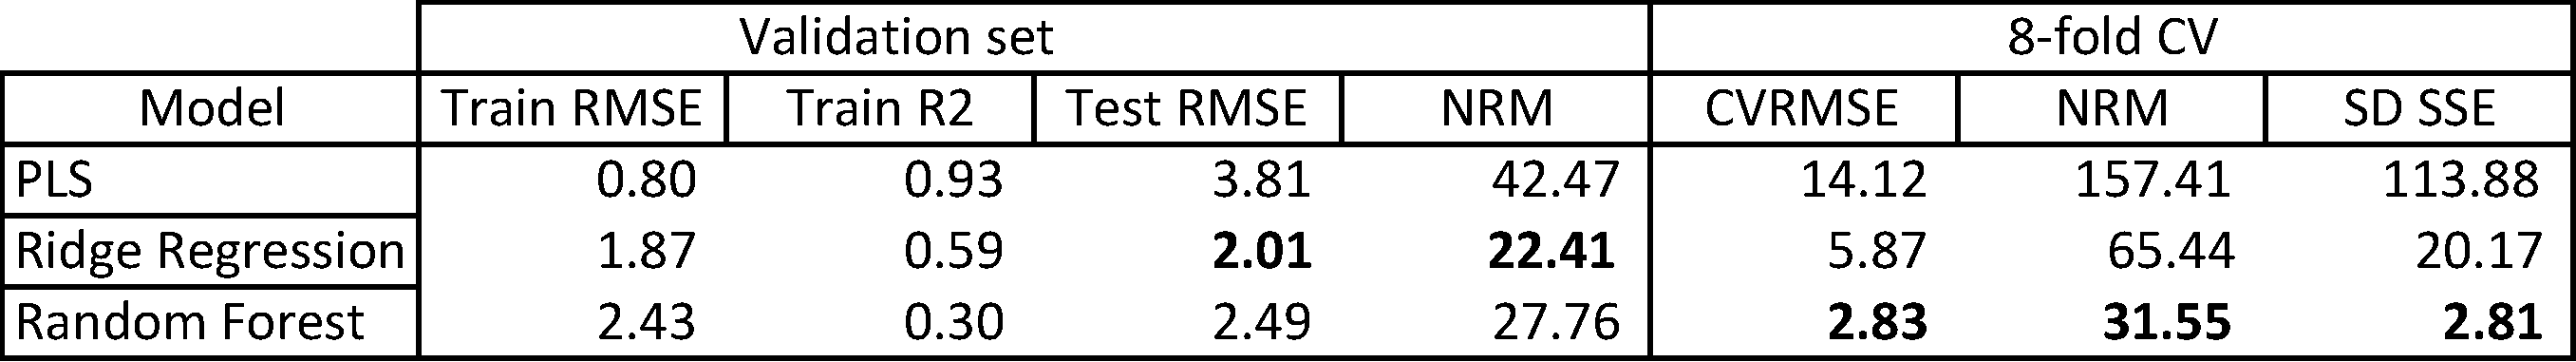
\includegraphics[width=1.8\columnwidth]{figures/test_sites/fig1.pdf}
	\label{fig:figure_placement}
\end{center}
\end{table*}

This study tests two other methods for overcoming the problem of collinearity in predicting nitrogen content of oats. Ridge regression (RR) and random forest regression (RF) are less common, but promising, methods on hyperspectral reflectance data \cite{Prasad2006,Caicedo2014,Imani2015}. RR uses penalisation and poses constraints on the predictor coefficients to reduce variance, using a $l_2$ norm. RF is a non-linear machine learning model. It uses bagging, an ensemble technique, to create many regression trees in parallel and combines these for a final higher performance model \cite{Breiman2001,Ismail2010}. Both models determine variable importance, which gives insight in important spectral regions for nitrogen content. Moreover, RF is able to capture non-linear behaviour.

I assess whether RR and non-linear RF models outperform PLSR in predicting the oat's nitrogen content by applying the models to the hyperspectral data used by Van Der Meij et al. (2017). I use the root mean square error of prediction (test RMSE) and the normalised RMSE (NRM) as a measure with a validation set. I assess the robustness of the models with 8-fold stratified cross-validation (CV). Lastly, I discuss the relative variable importance for each model to clarify the relation between nitrogen and reflectance.

\section{MATERIALS AND METHODS}

\subsection{Data and pre-processing}
The study area is located at Wageningen University \& Research, the Netherlands. This area consisted of 100 monoculture and 40 bi-culture plots (3x3m and 3x1.5m) in the growing season of 2014, half cultivated with oat (\textit{Aneva sativa}) and half with endive (\textit{Cichorium endiva}). In 2015, all plots were cultivated with oats and seven different plotwise treatments were applied. The plant samples for trait retrieval and the hyperspectral data were obtained around 1 July 2015, during the grain-filling stage. Nitrogen content was derived from the nitrogen concentration multiplied by the dry weight biomass. The spectral data was obtained using an octocopter UAV with a pushbroom spectrometer. Van Der Meij et al. (2017) discuss the details on the flight and calibration. The resulting data consists of contiguous band measurements from 450nm to 915nm, with intervals of 5nm. The spectral data for all plots were buffered to the inside to reduce edge-effects, and interpolated to result in one spectrum for each plot. Some plots violated the requirement of heterogeneity between the plots through the effects of different plot treatments. These were removed, resulting in a total of 56 plots used for the final analysis.


\subsection{Data analysis}

\subsubsection{Partial least squares regression} uses dimensionality reduction to deal with the collinearity in the hyperspectral data. Latent components decompose the dependent and the independent variables simultaneously by maximising the covariance between the two. This results in a number of latent vectors projected in a new space. Next, a linear regression is applied on the decomposed independent variables to predict the response. The amount of components that result in the lowest RMSE after leave-one-out CV is then used for prediction.

\subsubsection{Ridge regression} is similar to the OLS approach but uses a shrinkage penalty. RR seeks minimisation through shrinkage of the regression coefficients with the addition of a a $l_2$ norm. The tuning parameter $\lambda$ controls this penalty. Shrinkage increases with $\lambda$. Shrinkage improves on the OLS method for collinear predictors, as it reduces variance through its constraints. RR gives a solution for each value of $\lambda$, the optimal value is chosen for the lowest CV error using LOOCV on the training data. 

\subsubsection{Random forest regression} is a machine learning technique which uses ensemble learning. This consists of generating a vast amount of regression trees using the same algorithm in parallel. Each tree is generated using bootstrapped subsets of the data (bagging), called the bag. All trees combined result in a higher performing "forest". To ensure that the trees are not collinear with each other, only a certain number of random variables is considered at each node (split), called $mtry$. This parameter is chosen by the value that yields the lowest out-of-bag (OOB) error. This is the residual of predicted observations not used in creation of the tree, and is equivalent to LOOCV. The number of trees in the forest is set to 200, to ensure that the error rate has settled down. 


\subsubsection{Resampling methods} are tools that assess the prediction accuracy and variability of the model fits. I apply two different methods. Firstly, for the validation set approach, the data is split in a calibration set and a validation set. I apply the same random and equal split ($n = 28$) as proposed by \cite{VanDerMeij2017}. The models are fit on the hyperspectral UAV data of the calibration set, performance is measured by $R^2$ and RMSE on the in situ measured nitrogen content. To test the prediction accuracy, the model predicts the nitrogen content of the validation set, with the RMSEP as measure. Stratified 8-fold CV consists of splitting the data in 8 equal folds ($n = 7$), such that each fold is representative of the entire dataset through equal means. This ensures both bias and variance reduction. In iteration, each model fits 8 times to the 7 training folds, and predicts the nitrogen content for the held out validation fold. For each fit, the model parameters are re-estimated on the training folds. This artificially increases the rather sparse dataset and gives an estimate of the prediction variability. The obtained measures are sum of squared errors (SSE) of each iteration and the RMSE. The standard deviation of the total SSE, the mean of all RMSEs (CVRMSE) and the normalised CVRMSE (CVNRM) serve as a measure of prediction variability.

\subsubsection{Variable importance} finds the spectral regions that contribute most to the nitrogen prediction. For PLS, variable importance is computed using the absolute regression coefficients, weighted by their reduction of the total sum of squares. For RR, only the absolute values of the tuned coefficients are taken into account, not their contribution to reduction of the residuals. For RF, a variable's importance is measured by the difference in OOB error after removing that predictor from the tree. Since these three models use different algorithms and minimisation of different terms, it is difficult to use an absolute measure between them. I compute the scaled variable importance of each model and plot them together, to get insight in the relative important regions per model. Note that this is no absolute measure for inter-model comparison.

\begin{figure*}[ht!]
\begin{center}
		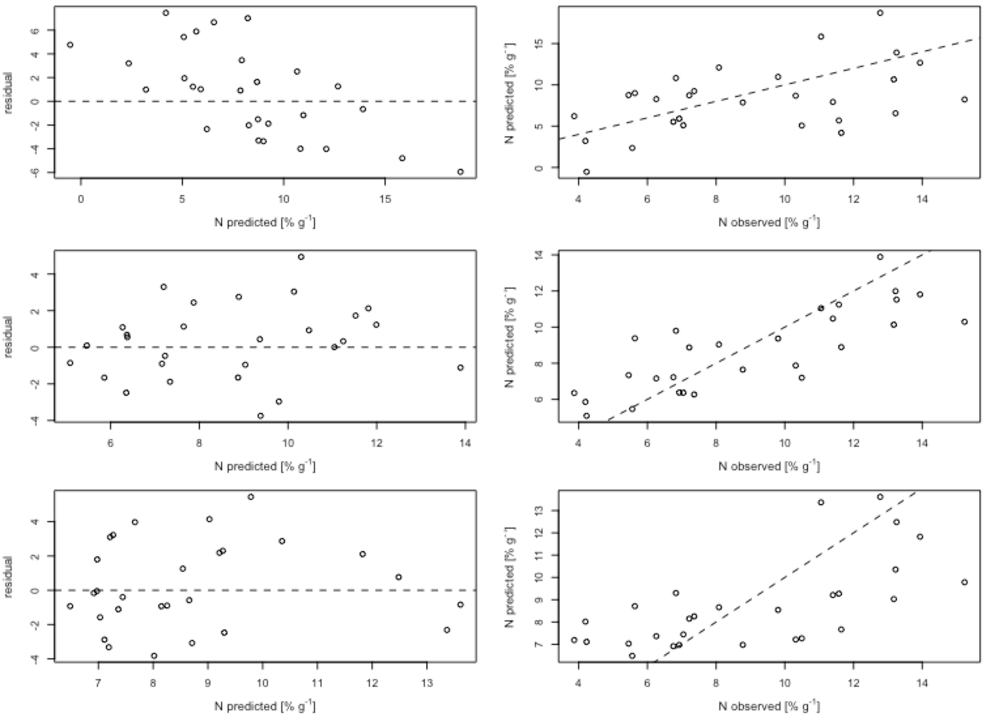
\includegraphics[width=2\columnwidth]{figures/test_sites/fig2.pdf}
	\caption{Residual plots (with 0 line) and scatterplots of predicted and observed nitrogen (with 1:1 line) on the validation set for the partial least squares model (top), ridge regression model (center) and random forest (bottom). (N: nitrogen).}
\label{fig:figure_placement}
\end{center}
\end{figure*}

\begin{figure}[ht!]
\begin{center}
		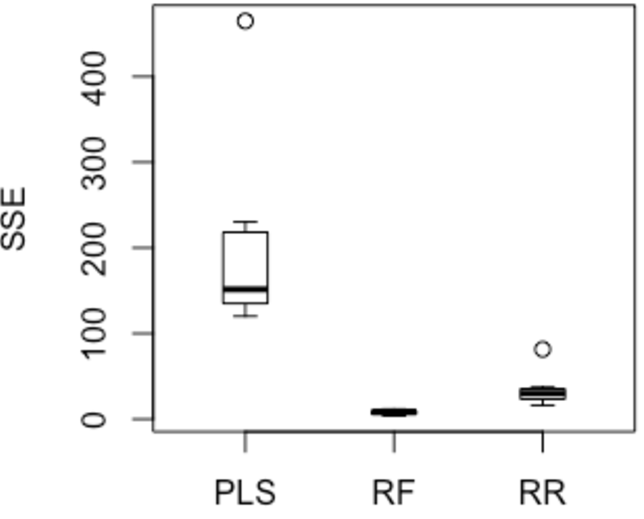
\includegraphics[width=0.7\columnwidth]{figures/test_sites/fig3.pdf}
	\caption{The spread of errors of stratified 8-fold cross validation for each fold. (SSE: sum of squared errors of prediction; PLS: partial least squares; RF: random forest; and RR: ridge regression).}
\label{fig:figure_placement}
\end{center}
\end{figure}

\begin{figure*}
\begin{center}
		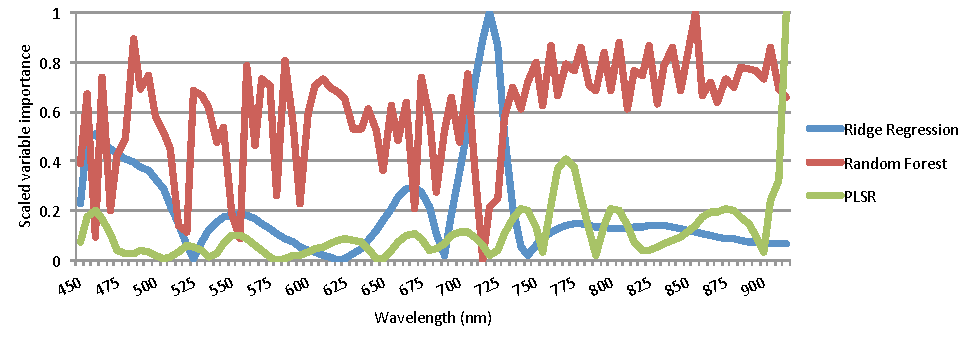
\includegraphics[width=1.8\columnwidth]{figures/test_sites/fig4.pdf}
	\caption{Scaled variable importance, computed with different methods for each model. This indicates the important spectral regions per model, but does not allow for numerical intercomparison.}
\label{fig:figure_placement}
\end{center}
\end{figure*}

\section{RESULTS}

The optimal number of latent components for PLS was 11 for the training data. As aforementioned, RF consisted of 200 trees and the optimal value of $mtry$ was 2. For RR, LOOCV resulted in a $\lambda$ of 3.72. Table 1 presents the results of the regressions. Performance on the training data was highly variable with $R^2$ values between 0.30 (RF) and 0.93 (PLS). As expected, the RMSE on the validation set was higher than the training set for PLS (+ 3.01), RR (+ 0.14) and RF (+ 0.06). Whereas PLS performed the best on the training data, it yielded the highest test RMSE (3.81). Its residuals also show a strong trend (Figure 2). RR is the best performing model on the test set (RMSE = 2.01), with a random residual plot.

The mean nitrogen content of the 8 folds used for cross validation was 8.99, with a standard deviation of 0.17. PLS yielded similar variant results, with the highest standard deviation of SSE (113) mainly influenced by one outlier (Figure 2). RF was the most robust model with a CVRMSE of 2.83 and standard deviation of SSE of 2.81, showing consistent performance. 

Figure 3 shows a high variance in trends between the models. Whereas RR and PLSR display rather smooth curves with clear peaks, the non-linear RF model shows spikes. PLS has many small peaks. There is a noticeable one in the blue (460nm), after which the next equivalent peak is positioned in the NIR, at the shoulder after the red edge (750nm). The strongest influence is around 775nm, and the highest importance occurs at the end of the range (915nm). RR shows 4 clear peaks: in the blue (460nm), green (560nm), end of the red (675) and the strongest influence is positioned on the red edge (725nm). Importance remains rather constant and non-zero for higher wavelengths. RF highlights some similar regions as PLSR (630nm, 710nm, 780nm, 810nm), but displays clear minimums at the peaks of PLS. The NIR region beyond the red edge is of constant relatively high importance, with a maximum at 860nm.
 



\section{DISCUSSION}

With the validation set approach both RR and RF outperform PLS on prediction of nitrogen content of oats using the entire hyperspectral reflectance. The optimised VI which yielded the highest predictive accuracy for nitrogen content by Van Der Meij et al. (2017) only performed slightly better (NRM -0.81\%). The high performance of PLS on the training data compared to its test RMSE indicates overfitting. Its variance is too high to explain unseen data. This is also evident from the standard deviation in 8-fold CV, in Table 1. Even though PLS is able to overcome the collinearity problem for sparse observations and high-dimensional data, variance and robustness is still a problem for small sample sizes \cite{Chung2010,Ji2015}. The difference in performance of RR and RF between the two methods shows that more observations are necessary to get good estimates of model performance. Even though RR performed best on the validation set, RF provides much higher accuracy for repeatedly sampled data (Figure 2). Another explanation for the poor performance of PLS might be non-linearity of the data, which the trend in the PLS residuals, Figure 1, indicates. The existence of a non-linear relationship would also explain why the RF model performs much better. RF does not assume linearity and is able to describe complex data and interactions between predictors. The high robustness of the RF model in 8-fold-CV is because of its ensemble learning. An individual regression tree would not obtain such accurate predictive power. It is the ensemble of 200 trees that adjusts for small errors in individual trees. The result is an increased prediction accuracy for unseen data, but at the cost of computation time.

The variable importance (Figure 3) around the red-edge is as expected. This is because of the known effect of leaf chlorophyll content and its link with nitrogen through photoynthesis \cite{Kooistra2016}. The different legacy treatments of the oat plots are only discriminable in their reflectance beyond 700nm. Van Der Meij et al. (2017) show a clear relation between treatment and nitrogen content. This explains the relatively constant and non-zero contribution of longer NIR wavelengths for all models. The contrast at 725nm between RR and RF is difficult to explain. It is possible that RR peaks there because of high importance of the neighbouring wavelengths. RF is not linear and does thus not show a smooth curve. Hence the neighbouring wavelengths have no influence at 725nm. RF is sometimes referred to as a black box, as it is hard to interpret the results. The variable importance of RF is a result of 200 non-linear trees and each tree considers two random predictors at each node split. It would therefore be interesting to explore different variable importance measures, and see their effects around 725nm \cite{Strobl2008}. The high contribution of the visible blue is interesting, since all indices developed for nitrogen characterisation consist of wavelengths in the visible green and beyond \cite{Mulla2013}. I find that nitrogen content may actually affect the visible blue, which is not registered by VIs as independent features. 

Future research could construct indices for plant nitrogen content including blue reflectances to confirm the results from this study. Furthermore, it should focus on regression models with feature selection to optimise the prediction accuracy and reduce overfitting \cite{Ji2015}. Using the entire spectrum gives insight in the important spectral regions, but noise reduction can improve the quality and confidence of these results. An example is sparse partial least squares, combining dimensionality reduction with feature selection, as demonstrated by Chung and Keles (2010). Furthermore, larger sample sizes will contribute to prediction accuracy, robustness and assessment of model quality. More observations will improve machine learning techniques and increase the number of methods that can be applied. This can lead to better insights in the spectral influence of plant nitrogen content and confirm non-linear behaviour. Additionally, larger sample sizes would increase the reliability of the data, as the in situ nitrogen content measurements from samples were considered to be representative of the entire plot \cite{VanDerMeij2017}. 

\section{CONCLUDING REMARKS}
Exploring variable importance is crucial for plant nitrogen content since its relation with reflectance is still poorly understood. Partial least squares regression (PLS) is used widely in hyperspectral multivariate analysis to assess important spectral regions. I show that both ridge regression (RR) and random forest regression (RF) outperform the PLS model for predicting oat nitrogen content. There is great potential in improving the models through feature selection, more observations and advanced variable importance assessment. The ability to predict plant nitrogen content using the visible blue region should be explored.


\nocite{*}
\vspace{4mm}

\bibliography{AEO} 

\vspace{1cm}

\end{document}
